\section{Collisions}
\label{sec:dsmc_collisions_model}
In a particle simulation with a continuous force field it is not clear how one would define a \textit{collision event}. If two equal atoms with the same velocity move towards each other, the atoms would at some point reverse their velocities. In this case, one could define the collision event to occur at \textit{the time of which their relative distance is at its minimum}, but other, equally valid, definitions probably exists. It is however clear that a collision should be identified as an event that happens when the atoms are close, i.e. short ranged forces.\\
As we already have mentioned, we don't operate with forces in the DSMC model. We calculate collision rates from the kinetic theory. In order to do so, we do need to choose an underlying collision model from which we will calculate the collision rates. We have chosen the \textit{hard sphere} model, where each particle is assumed to be a perfect hard sphere with diameter $d$ and mass $m$. Hard sphere means that two particles with radius $R_1$ and $R_2$ will undergo an \textit{fully elastic} collision if their relative distance equals the sum of their radii, see figure \ref{fig:dsmc_hard_sphere}. In DSMC, we will then apply what we could call a stochastic hard sphere collision model, where we use the hard sphere model only to calculate the statistical collision rates.\\
\begin{figure}[h]
\begin{center}
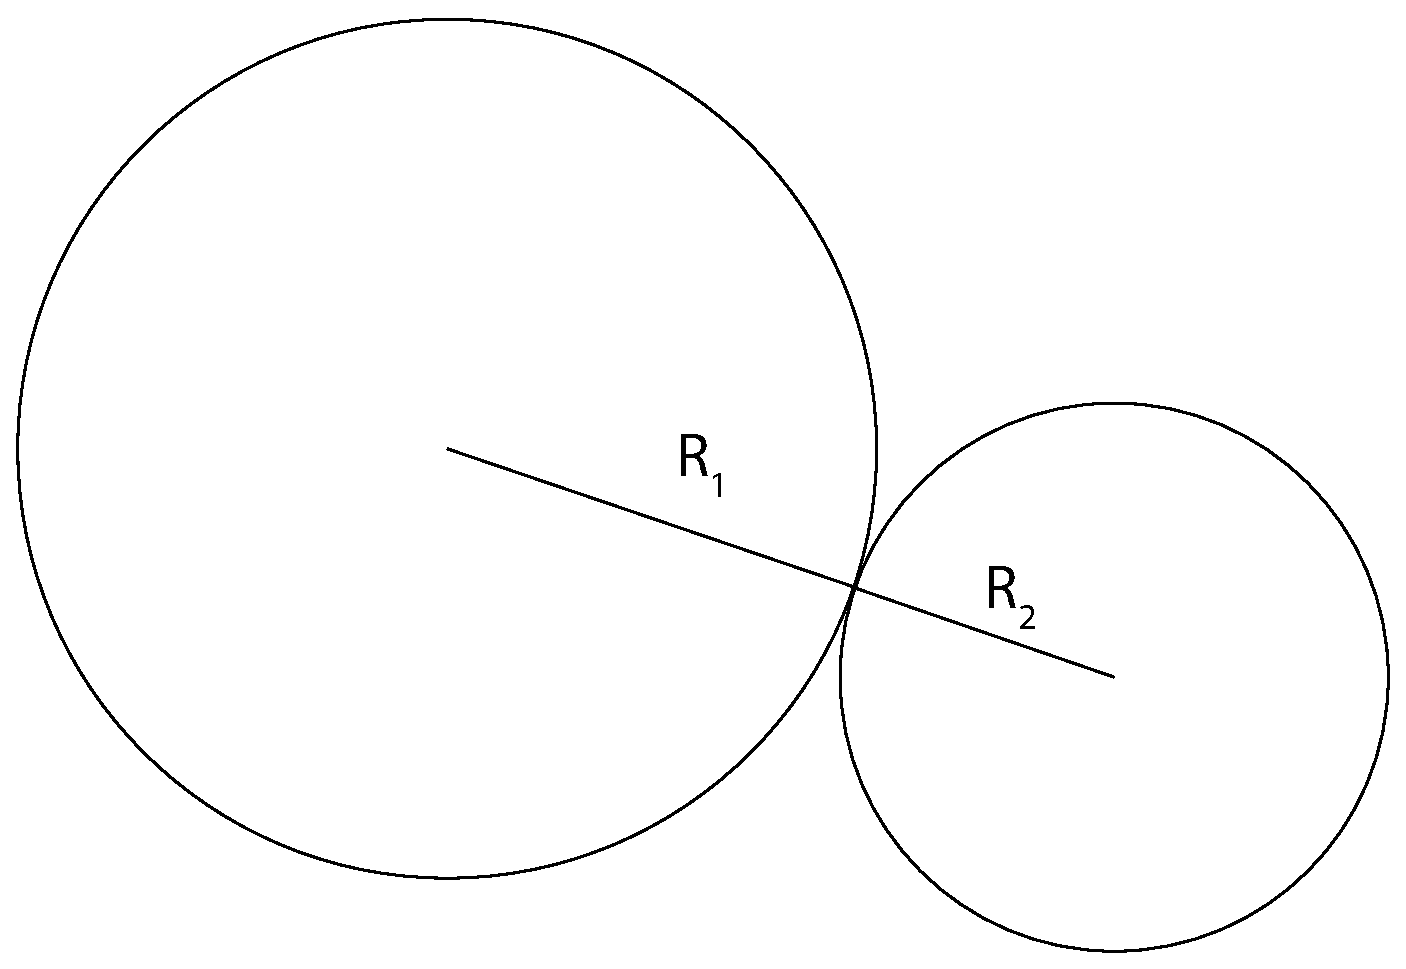
\includegraphics[width=0.5\textwidth, trim=0cm 0cm 0cm 0cm, clip]{DSMC/figures/collisions.eps}
\end{center}
\caption{The hard sphere collision model. Two particles will collide if their relative distance becomes smaller than $R_1+R_2$.}
\label{fig:dsmc_hard_sphere}
\end{figure}
Since collisions should occur to nearby particles only, we sort the particles into spatial cells, allowing only particles from the same cell to collide. The dimension of these cells should not exceed the mean free path. If this was the case, two particles displaced by a distance larger than the mean free path could transfer momentum or energy faster than what would happen in a real gas (collisions usually transfer energy and momentum). Note that we allow particles \textit{moving away} from each other to collide, since the simulated particles should not be interpreted as real molecules or atoms. In some sense, they are quasi-particles carrying statistical information only. They can be interpreted as density packets representing the distribution function $f$ from section \ref{sec:kinetic_theory_distribution_function}. Now that we have chosen a collision model, we should compute the collision rates.
\subsection{Number of collisions}
We will here use similar arguments as we did deriving the mean free path in section \ref{sec:mean_free_path_calculation}. If we choose two particles, $i$ and $j$, with relative velocity $\vec v_r$, each representing $N_\text{eff}$ real atoms with effection collision area $A=\pi d^2$ (see section \ref{sec:mean_free_path_calculation}), in a collision cell with volume $V_c$, the total volume sweeped out during a timestep is
\begin{align}
	V_\text{sweep} = N_\text{eff}\pi d^2v_r\Delta t.
\end{align}
The probability that they will collide is the total sweeped volume $V_\text{sweep}$ divided by the total cell volume $V_c$
\begin{align}
	P_\text{coll} = \frac{N_\text{eff}\pi d^2 v_r\Delta t}{ V_c}.
\end{align}
If a collision cell has $N_c$ particles, a particle has $(N_c-1)$ potential collision partners. So the total number of collision pairs (we divide by two to prevent double counting of pairs) is $N_c(N_c-1)/2$ which gives the number of collisions $M_\text{coll}$
\begin{align}
	\label{eq:dsmc_number_of_collisions}
	M_\text{coll} = \frac{N_c(N_c-1)}{2}P_\text{coll} = \frac{N_c(N_c-1)N_\text{eff}\pi d^2\langle v_r \rangle \Delta t}{2 V_c},
\end{align}
where we replaced the relative velocity $v_r$ by the mean value in the cell
\begin{align}
	\langle v_r \rangle = \frac{1}{N_c} \sum_{i>j} |\vec v_i - \vec v_j|.
\end{align}
But computing the mean relative velocity $\langle v \rangle$ in each cell \textit{every timestep} sounds like a horrendous thing to do. It requires to sum over all pairs which is $O(N^2)$, which is exactly what we try to avoid in the first place. But we can do a little trick. Instead, we calculate $M_\text{cand}$ \textit{candidate pairs} so that
\begin{align}
	\frac{M_\text{coll}}{M_\text{cand}} = \frac{\langle v_r\rangle}{v_r^\text{max}},
\end{align}
since the probability of collision is proportional to the relative velocity. Each of these candidates go through an acceptance-rejection process where we pick a uniform random number $\mathcal{R}_1\in (0,1)$ and accept the collision if
\begin{align}
	v_r \leq v_r^\text{max}\mathcal{R}_1.
\end{align}
This will only accept $\langle v_r\rangle/v_r^\text{max}$ of the candidates and we end up with $M_\text{coll}$ actual collisions, as desired. The number of candidate pairs is then computed as
\begin{align}
	M_\text{cand} = \frac{N_c(N_c-1)N_\text{eff}\pi d^2v_r^\text{max} \Delta t}{2V_c}.
\end{align}
If we choose $v_r^\text{max}$ very high, we will still perform the correct amount of collisions, but the number of rejected collisions would be high and hence the algorithm is inefficient. If a collision pair has a higher relative velocity, we simply update this variable (in that cell).\\
We should one more time mention that particles moving away from each other can collide. This property has, as we will see in section \ref{sec:dsmc_eos}, an interesting consequence leading to the ideal gas equation of state. One more thing, we haven't figured out how to perform the actual collisions. Until now, we know only how to select collision pairs, so let's calculate the post-collision velocities.
\subsection{Post-collision velocities}
After a collision is accepted, we want to choose new velocities conserving both energy and momentum. We need a total of six equations to determine the post-collision velocities, where four are provided through the conservation laws. Conservation of momentum reveals that the center of mass velocity is unchanged
\begin{align}
	\vec v_\text{cm} = \frac{1}{2}(\vec v_i + \vec v_j) = \frac{1}{2}(\vec v_i^* + \vec v_j^*) = \vec v_\text{cm}^*,
\end{align}
where the energy conservation tells us that the relative velocity vector does not change its magnitude
\begin{align}
	v_r = |\vec v_i - \vec v_j| = |\vec v_i^* - \vec v_j^*| = v_r^*.
\end{align}
Here we used that the velocities of the particles are uncorrelated so that $\vec v_i\cdot\vec v_j = 0$ on average. The two remaining degrees of freedom are determined by choosing the direction of the relative velocity
\begin{align}
	\vec v_r^* = v_r\left[(\sin\theta\cos\phi)\vec i + (\sin\theta\sin\phi) \vec j + (\cos\theta)\vec k\right],
\end{align}
where the angles are uniformly distributed over the unit sphere so that all directions for the relative velocity are equally probable. The area element $\dm\Omega$ can be written as
\begin{align}
	\dm\Omega = \sin\theta\,\dm\theta\,\dm\phi = -\dm\phi\,\dm(\cos\theta),
\end{align}
so we need to choose $\phi$ and $\cos\theta$ uniformly. This is easy, we simply choose 
\begin{align*}
	\phi = 2\pi\mathcal{R}_2 & \qquad \qquad \cos\theta = 2\mathcal{R}_3 - 1,
\end{align*}
where $\mathcal{R}_2$ and $\mathcal{R}_3$ are random numbers in the range $(0,1)$ and calculate $\sin\theta = \sqrt{1 - \cos^2\theta}$. The post-collisions velocities are then found by
\begin{align}
	\vec v_i^* &= \vec v_\text{cm} + \frac{1}{2}\vec v_r^*\\
	\vec v_j^* &= \vec v_\text{cm} - \frac{1}{2}\vec v_r^*.
\end{align}
An example of how this can be implemented is found in listing \ref{lst:post_collisions_velocities}.
\begin{lstlisting}[caption=Example code showing how to determine post-collision velocities., label=lst:post_collisions_velocities]
void collide_molecules(Vector3 &v0, Vector3 &v1, Random &rnd) {
    Vector3 v_center_of_mass = 0.5*(v0 + v1);
    double v_rel = (v1 - v2).length();
    
    double cos_theta = 1.0 - 2.0*rnd.next_double();
    double sin_theta = sqrt(1.0 - cos_theta*cos_theta);
    double phi = 2*M_PI*rnd.next_double();

    Vector3 relative_velocity(1,1,1)*v_rel;
    relative_velocity.x *= cos_theta;
    relative_velocity.y *= sin_theta*cos(phi);
    relative_velocity.z *= sin_theta*sin(phi);
    v0 = v_center_of_mass + 0.5*relative_velocity;
    v1 = v_center_of_mass - 0.5*relative_velocity;
}
\end{lstlisting}